\documentclass[aspectratio=169]{beamer}
\usepackage{amsmath}
\usepackage{amssymb}
\usepackage{minted}
\usepackage{graphicx}
\title{Kernel Density Estimation}
\subtitle{Assignment 1}
\author{Lucas Støjko Andersen}
\setminted{fontsize=\fontsize{8pt}{8pt}}
\institute{University of Copenhagen}
\date{\today}
\begin{document}
\begin{frame}
    \titlepage
\end{frame}
\begin{frame}
    \frametitle{Kernel Density Estimation}
    \framesubtitle{Kernels}
    Let $K:\mathbb{R}\longrightarrow[0,\infty)$ with properties
    \begin{align}
      &K(x)=K(-x),\quad\forall x\in\mathbb{R}\\
      &1 = \int_{\mathbb{R}}K(x)dx
    \end{align}
    and $X_{1},X_{2},\ldots X_{n}$ be random variables with density $f$. Then 
    \begin{equation}
      \hat{f}(x)=\frac{1}{n\lambda}\sum_{i=1}^{n}K\left(\frac{x - x_{i}}{\lambda}\right)
    \end{equation}
    is the kernel density estimate of $f$ with bandwidth $\lambda > 0$ and kernel $K$.
\end{frame}
\begin{frame}[fragile]
  \frametitle{Implementation of Kernel Density Estimate}
\begin{minted}{r}
R_dens_for <- function(x, p, kernel, bandwidth) {
  m <- length(p)
  n <- length(x)
  result <- numeric(m)
  for(i in 1:m) {
    for(j in 1:n) {
      result[i] <- result[i] + kernel((p[i] - x[j]) / bandwidth)
    }
  }
  result / (n * bandwidth)
}
\end{minted}
\end{frame}
\begin{frame}[fragile]
  \frametitle{Testing the Implementation}
  \framesubtitle{Epanechnikov Kernel}
  Use the kernel density estimate on the \textit{epanechnikov} kernel given by
  \begin{equation}
    K(x)=\frac{3}{4}(1 - x^{2})1_{[0,1]}(x).
  \end{equation}
  Implemented in \texttt{R} as\\[5pt]
\begin{minted}{r}
e_kernel <- function(x) {
  0.75 * (1 - x^2) * (abs(x) <= 1)
}
\end{minted}
\end{frame}
\begin{frame}[fragile]
  \frametitle{The Test Case}
  \framesubtitle{Gaussian Mixture}
\begin{minted}{r}
x <- c(rnorm(200, -1, 0.1), 
       rnorm(200, -0.5, 0.1),
       rnorm(200, 0, 0.3),
       rnorm(200, 0.5, 0.7),
       rnorm(200, 1, 1))

funky_density <- function(x) {
  dnorm(x, -1, 0.1) / 5 +
    dnorm(x, -0.5, 0.1) / 5 +
    dnorm(x, 0, 0.3) / 5 +
    dnorm(x, 0.5, 0.7) / 5 +
    dnorm(x, 1, 1) / 5
}
\end{minted}
\end{frame}
\begin{frame}
  \frametitle{Plotting the Densities}
  With $\lambda = 0.1$ we plot the estimated density together with \texttt{R}'s default \texttt{density} implementation and the true density.
  \begin{figure}
    \centering
    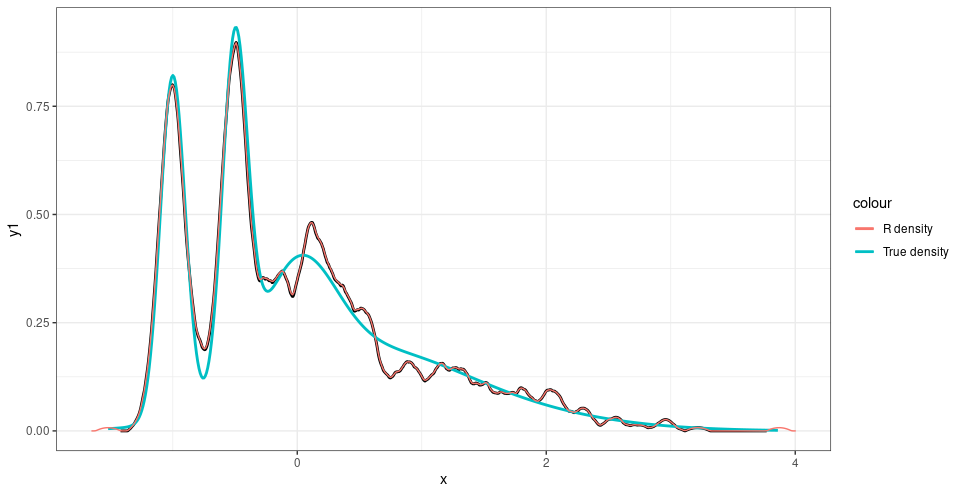
\includegraphics[scale = 0.4]{figure/FirstTest.png}
  \end{figure} 
\end{frame}
\begin{frame}
  \frametitle{Bandwidth Selection}
  \framesubtitle{Leave-One-Out Cross Validation}  
  We persue bandwidth selection through leave-one-out cross validation. Let
  \begin{equation}
    \hat{f}^{-i}_{\lambda}=\frac{1}{(n-1)\lambda}\sum_{j\neq i}^{n}K\left(\frac{x_{i}-x_{j}}{\lambda}\right).
  \end{equation}
  We then select the bandwidth
  \begin{equation}
    \hat{\lambda}_{\text{CV}}=\underset{\lambda > 0}{\arg\,\max}\sum_{i=1}^{n}\log\hat{f}^{-i}_{\lambda}.
  \end{equation}
\end{frame}
\begin{frame}[fragile]
  \frametitle{Implementation of LOOCV Bandwidth Selection}
  \framesubtitle{Bandwidth Selection and Oracle Bandwidth as Comparison}
\begin{minted}{r}
bw_cv_R2 <- function(x, kernel, max_bw = 2) {
  cv_func <- function(l) {
    if(l < .Machine$double.eps) Inf
    n <- length(x)
    K <- numeric(n)
    for(i in 1:n) {
      K[i] <- sum(kernel((x[i] - x[-i]) / l))
    }
    cv <- sum(log(K[K > .Machine$double.eps]))
    n * log((n - 1) * l) - cv
  }
  suppressWarnings(optimize(cv_func, c(0, max_bw)))$minimum
}

bw_oracle <- function(x, kernel) {
  n <- length(x)
  K <- integrate(function(x) kernel(x)^2, -Inf, Inf)$value
  sigma2 <- integrate(function(x) kernel(x) * x^2, -Inf, Inf)$value
  sigma <- min(sd(x), IQR(x) / 1.34)
  (8 * sqrt(pi) * K / (3 * sigma2^2))^(1/5) * sigma * n^(-1/5)
}
\end{minted}
\end{frame}
\begin{frame}[fragile]
  \frametitle{Implementation of Kernel Density Estimate with Bandwidth Selection}
\begin{minted}{r}
dens_R1 <- function(x,
                   kernel,
                   bandwidth,
                   ...,
                   points = 512L) {
  if(is.function(bandwidth)) {
    bw <- bandwidth(x, kernel, ...)
  } else {
    bw <- bandwidth
  }
  p <- seq(min(x) - bw, max(x) + bw, length.out = points)
  y <- R_dens_for(x, p, kernel, bw)
  structure(
    list(
      x = p,
      y = y,
      bw = bw
    ),
    class = "dens"
  )
}
\end{minted}
\end{frame}
\begin{frame}
  \frametitle{Plotting the Density Estimate with Bandwidth Selection}
  The LOOCV bandwidth is $0.1155167$ and the oracle bandwidth is $0.4746436$.
  \begin{figure}
    \centering
    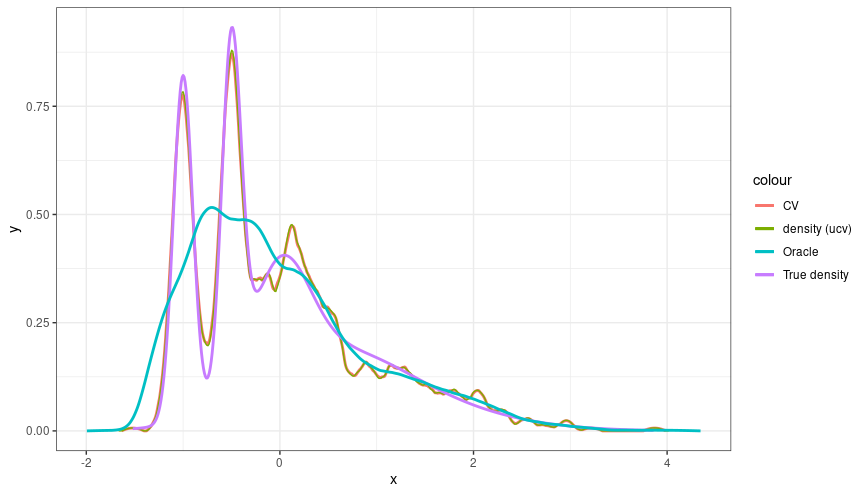
\includegraphics[scale = 0.5]{figure/application.png}
  \end{figure}
\end{frame}
\begin{frame}[fragile]
  \frametitle{Profiling the Implementation}
  \framesubtitle{Profiling the Kernel Density Estimation}
  \begin{figure}
    \centering
    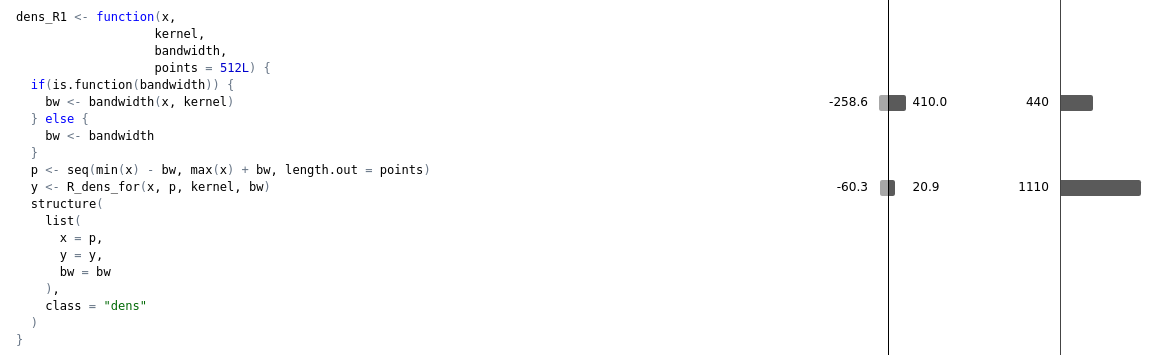
\includegraphics[scale = 0.35]{figure/density_profile.png}
  \end{figure}
\end{frame}
\begin{frame}[fragile]
  \frametitle{Profiling the Implementation}
  \framesubtitle{Profiling the Bandwidth Selection}
  \begin{figure}
    \centering
    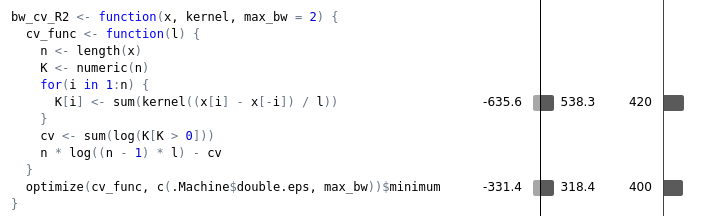
\includegraphics[scale = 0.35]{figure/BW_profile.png}
  \end{figure}
\end{frame}
\begin{frame}[fragile]
  \frametitle{Alternative Implementations of Calculating the Density Estimate}
\begin{minted}[fontsize = \fontsize{7pt}{7pt}]{r}
R_dens <- function(x, p, kernel, bandwidth) {
  m <- length(p)
  n <- length(x)
  result <- numeric(m)
  for(i in 1:m) {
    result[i] <- sum(kernel((p[i] - x) / bandwidth))
  }
  result / (n * bandwidth)
}

R_dens_for <- function(x, p, kernel, bandwidth) {
  m <- length(p)
  n <- length(x)
  result <- numeric(m)
  for(i in 1:m) {
    for(j in 1:n) {
      result[i] <- result[i] + kernel((p[i] - x[j]) / bandwidth)
    }
  }
  result / (n * bandwidth)
}

R_dens_apply <- function(x, p, kernel, bandwidth) {
  app_func <- function(t) sum(kernel((t - x) / bandwidth))
  result <- sapply(p, app_func)
  result / (length(x) * bandwidth)
}
\end{minted}
\end{frame}
\begin{frame}
  \frametitle{Benchmarking Alternative Implementations using \texttt{bench} Package}
  \framesubtitle{Plot}
  \begin{figure}
    \centering
    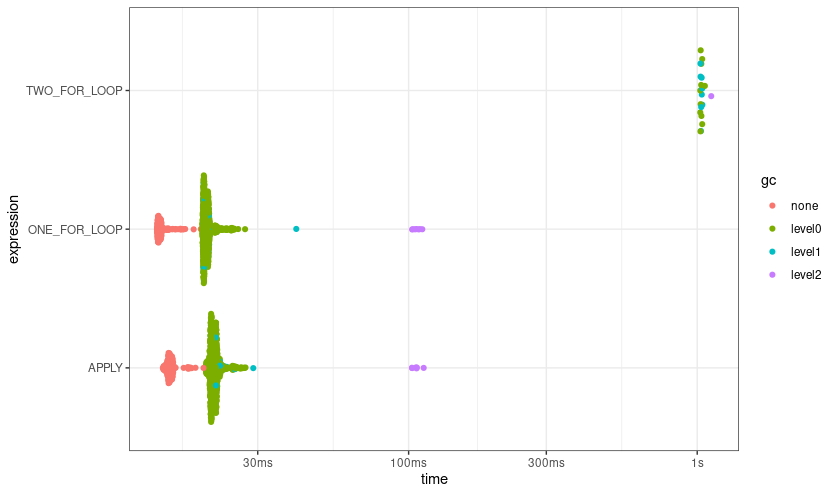
\includegraphics[scale = 0.5]{figure/ForVsApply.png}
  \end{figure}
\end{frame}
\begin{frame}
  \frametitle{Benchmarking Alternative Implementations using \texttt{bench} Package}
  \framesubtitle{Table}
  \begin{figure}
    \centering
    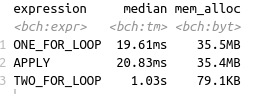
\includegraphics[scale = 0.7]{figure/R_FOR_APPLY_dens.png}
  \end{figure}
\end{frame}
\begin{frame}[fragile]
  \frametitle{Alternative LOOCV Implementations}
  Let $K_{i,j}=K((x_{i}-x_{j}) / \lambda)$ and notice $K_{i,j}=K_{j,i}$.\\
\begin{minted}{r}
bw_cv_R <- function(x, kernel, max_bw = 2) {
  cv_func <- function(l) {
    if(l < .Machine$double.eps) Inf
    n <- length(x)
    K <- numeric(n)
    for(i in 2:n) {
      index <- 1:(i - 1)
      tmp <- kernel((x[i] - x[index]) / l)
      K[i] <- K[i] + sum(tmp)
      K[index] <- K[index] + tmp[index]
    }
    cv <- sum(log(K[K > .Machine$double.eps]))
    n * log((n - 1) * l) - cv
  }
  suppressWarnings(optimize(cv_func, c(0, max_bw)))$minimum
}
\end{minted}
\end{frame}
\begin{frame}
  \frametitle{Alternative LOOCV Implementation Benchmarks}
  \framesubtitle{Plot}
  \begin{figure}
    \centering
    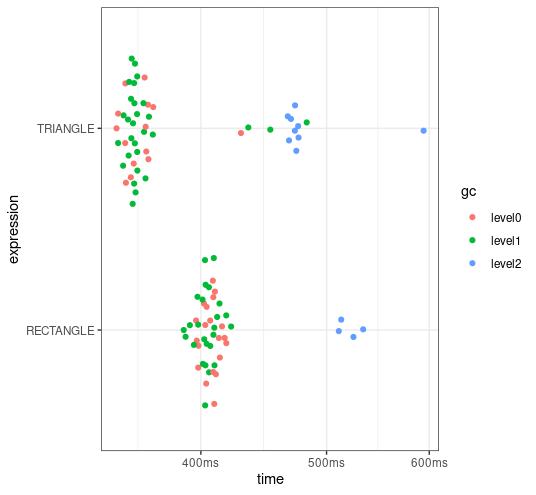
\includegraphics[scale = 0.5]{figure/RecVsTri.png}
  \end{figure}
\end{frame}
\begin{frame}
  \frametitle{Alternative LOOCV Implementation Benchmarks}
  \framesubtitle{Table}
  \begin{figure}
    \centering
    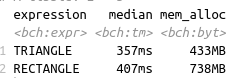
\includegraphics[scale = 0.7]{figure/TRIANGLE_RECTANGLE.png}
  \end{figure}
\end{frame}
\begin{frame}[fragile]
  \frametitle{Improving Further with \texttt{RCPP} Package} 
  \framesubtitle{Implementing the kernel in \texttt{RCPP}}
  Implementing the kernel in \texttt{RCPP} could improve performance per the profiling.\\
\begin{minted}{cpp}
// [[Rcpp::export]]
NumericVector e_kernel_cpp(NumericVector x) {
  int n = x.size();
  NumericVector result(n);
  for(int i = 0; i < n; ++i)
    result[i] = std::abs(x[i]) <= 1 ? 0.75 * (1 - x[i] * x[i]) : 0;
  return result;
}
\end{minted}
\end{frame}
\begin{frame}[fragile]
  \frametitle{Improving Further with \texttt{RCPP} Package}
  \framesubtitle{Calling Kernel from \texttt{R} in \texttt{RCPP}} 
\begin{minted}{cpp}
// [[Rcpp::export]]
NumericVector dens_rcpp_partial(NumericVector x,
                                Function kernel,
                                double bandwidth,
                                NumericVector points) {
  int n = x.size(), m = points.size();
  NumericVector result(m);
  for(int i = 0; i < m; ++i) {
    NumericVector call = kernel((points[i] - x) / bandwidth);
    result[i] = sum(call) / (n * bandwidth);
  }
  return result;
}
\end{minted}
\end{frame}
\begin{frame}[fragile]
  \frametitle{Improving Further with \texttt{RCPP} Package}
  \framesubtitle{Calling Kernel from \texttt{R} in \texttt{RCPP}}
\begin{minted}{cpp}
// [[Rcpp::export]]
double bw_cv_rcpp_partial(NumericVector x,
                          Function kernel,
                          double bandwidth) {
  int n = x.size();
  NumericVector K(n);
  double result;
  for(int i = 1; i < n; ++i) {
    Range r = Range(0, i - 1);
    NumericVector tmp = kernel((x[r] - x[i]) / bandwidth);
    for(int j = 0; j < i; ++j)
      K[j] += tmp[j], K[i] += tmp[j];
      
  }
  for(int s = 0; s < n; ++s)
    if(K[s] > std::numeric_limits<double>::min()) result += std::log(K[s]);
  return n * log((n - 1) * bandwidth) - result;
}
\end{minted} 
\end{frame}
\begin{frame}[fragile]
  \frametitle{Improving Further with \texttt{RCPP} Package}
  \framesubtitle{Full \texttt{RCPP} Implementation}  
\begin{minted}{cpp}
// [[Rcpp::export]]
NumericVector dens_rcpp(NumericVector x,
                        double bandwidth,
                        NumericVector points) {
  int n = x.size(), m = points.size();
  NumericVector result(m);
  for(int i = 0; i < m; ++i) {
    NumericVector call = e_kernel_cpp((points[i] - x) / bandwidth);
    result[i] = sum(call) / (n * bandwidth);
  }
  return result;
}
\end{minted}
\end{frame}
\begin{frame}[fragile]
  \frametitle{Improving Further with \texttt{RCPP} Package}
  \framesubtitle{Full \texttt{RCPP} Implementation}
\begin{minted}{cpp}
// [[Rcpp::export]]
double bw_cv_rcpp(NumericVector x,
                  double bandwidth) {
  int n = x.size();
  NumericVector K(n);
  double result;
  for(int i = 1; i < n; ++i) {
    Range r = Range(0, i - 1);
    NumericVector tmp = e_kernel_cpp((x[i] - x[r]) / bandwidth);
    for(int j = 0; j < i; ++j)
      K[j] += tmp[j], K[i] += tmp[j];
  }
  for(int s = 0; s < n; ++s)
    if(K[s] > std::numeric_limits<double>::min()) result += std::log(K[s]);
  return n * std::log((n - 1) * bandwidth) - result;
}
\end{minted}
\end{frame}
\begin{frame}
  \frametitle{Benchmarking \texttt{RCPP} Density Calculation}
  \framesubtitle{Plot}
  \begin{figure}
    \centering
    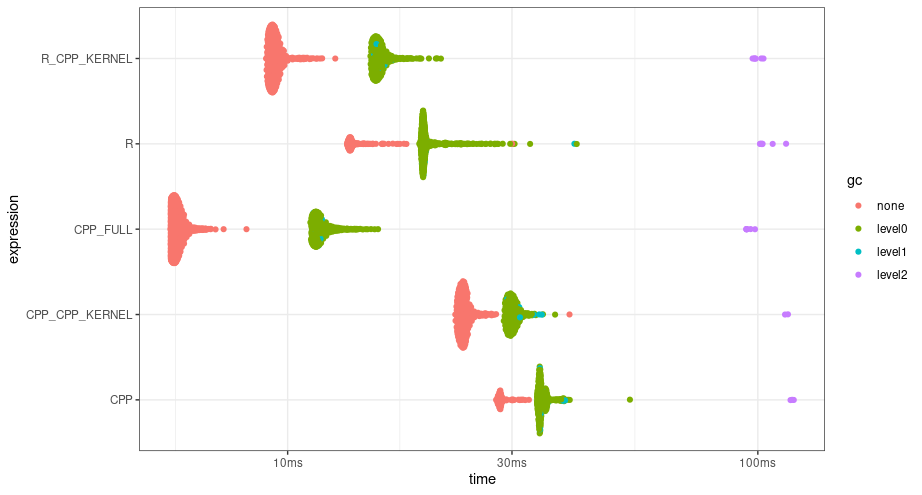
\includegraphics[scale = 0.5]{figure/RcppVsRDens.png}  
  \end{figure}
\end{frame}
\begin{frame}
  \frametitle{Benchmarking \texttt{RCPP} Density Calculation}
  \framesubtitle{Table}
  \begin{figure}
    \centering
    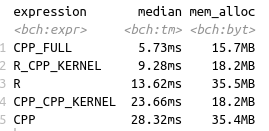
\includegraphics[scale = 0.7]{figure/table_R_RCPP_dens.png}  
  \end{figure}
\end{frame}
\begin{frame}
  \frametitle{Benchmarking \texttt{RCPP} Bandwidth Selection}
  \framesubtitle{Plot}
  \begin{figure}
    \centering
    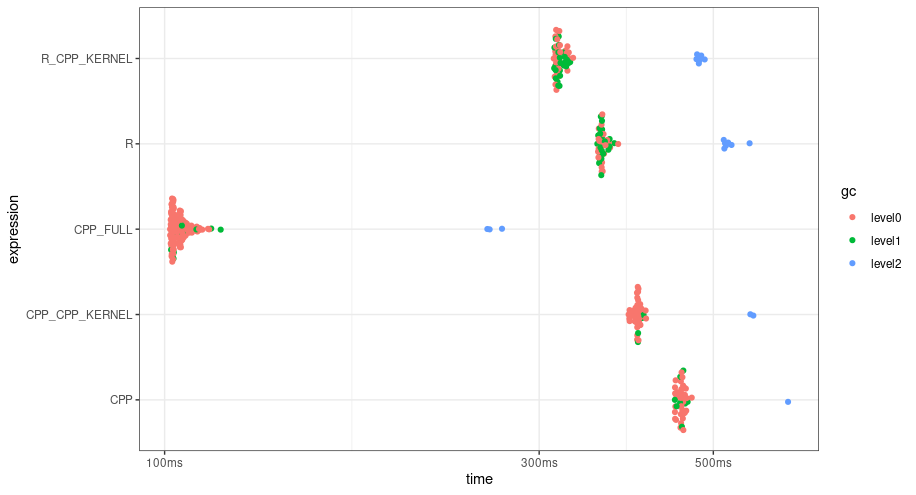
\includegraphics[scale = 0.5]{figure/RCPP_R_CV.png}  
  \end{figure}
\end{frame}
\begin{frame}
  \frametitle{Benchmarking \texttt{RCPP} Bandwidth Selection}
  \framesubtitle{Table}
  \begin{figure}
    \centering
    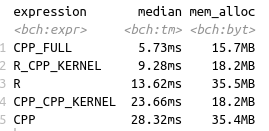
\includegraphics[scale = 0.7]{figure/table_R_RCPP_dens.png}  
  \end{figure}
\end{frame}
\begin{frame}[fragile]
  \frametitle{Improving Further Using \texttt{R}'s C API}
  \framesubtitle{Implementation of Density Calculation} 
\begin{minted}{c}
#include <Rinternals.h>
#include <R.h>

SEXP C_dens(SEXP x, SEXP p, SEXP kernel, SEXP bw, SEXP rho) {
  int n = length(x), m = length(p); 
  SEXP dens = PROTECT(allocVector(REALSXP, m));
  SEXP tmp = PROTECT(allocVector(REALSXP, n));
  SEXP K_Call = PROTECT(lang2(kernel, R_NilValue));
  double *x_ = REAL(x), *p_ = REAL(p), *tmp_ = REAL(tmp), *dens_ = REAL(dens);
  double bw_ = REAL(bw)[0];
  
  memset(dens_, 0, sizeof(double) * m);
  
  for(int i = 0; i < m; ++i) {
    for(int j = 0; j < n; ++j)
      tmp_[j] = (p_[i] - x_[j]) / bw_;
    SETCADR(K_Call, tmp);
    SEXP result = eval(K_Call, rho);
    double *result_ = REAL(result);
    for(int j = 0; j < n; ++j)
      dens_[i] += result_[j];
    dens_[i] /= n * bw_;
  }
  UNPROTECT(3);
  return dens;
}
\end{minted}
\end{frame}
\begin{frame}[fragile]
  \frametitle{Improving Further Using \texttt{R}'s C API}
  \framesubtitle{Implementation of LOOCV}
\begin{minted}[fontsize = \fontsize{6.5pt}{6.5pt}]{c}
#include <Rinternals.h>
#include <R.h>
#include <float.h>

SEXP C_cv(SEXP x, SEXP fn, SEXP lambda, SEXP rho) {
  if(REAL(lambda)[0] < DBL_EPSILON) return ScalarReal(INFINITY);
  int n = length(x);
  SEXP K = PROTECT(allocVector(REALSXP, n));
  SEXP fn_call = PROTECT(lang2(fn, R_NilValue));
  SEXP out = PROTECT(ScalarReal(0.0));
  double *x_ = REAL(x), *K_ = REAL(K), *out_ = REAL(out);
  double h_ = REAL(lambda)[0];
  memset(K_, 0, sizeof(double) * n);
  for(int i = 1; i < n; ++i) {
    SEXP tmp = PROTECT(allocVector(REALSXP, i));
    double *tmp_ = REAL(tmp);
    for(int k = 0; k < i; ++k)
      tmp_[k] = (x_[i] - x_[k]) / h_;
    SETCADR(fn_call, tmp);
    SEXP s = eval(fn_call, rho);
    double *s_ = REAL(s);
    UNPROTECT(1);
    for(int j = 0; j < i; ++j) {
      K_[i] += s_[j];
      K_[j] += s_[j];
    }
  }
  for(int i = 0; i < n; ++i)
    if(K_[i] > DBL_EPSILON) *out_ += log(K_[i]);
  *out_ = n * log((n - 1) * h_) - (*out_);
  UNPROTECT(3);
  return out;
}
\end{minted}
\end{frame}
\begin{frame}[fragile]
  \frametitle{Improving Further Using \texttt{R}'s C API}  
  \framesubtitle{Calling the C Code}
  Compile to shared library using \texttt{R CMD SHLIB} command. If used in a package a little more work is required. For now just used \texttt{dyn.load} function in \texttt{R} to link the shared library.\\

\begin{minted}{r}
bw_cv <- function(x, kernel, max_bw = 2) {
  cv_func <- function(l) .Call("C_cv", x, kernel, l, environment())
  suppressWarnings(optimize(cv_func, c(0, max_bw)))$minimum
}
\end{minted}
\end{frame}
\begin{frame}
  \frametitle{Benchmarking All Density Calculation Implementations}
  \framesubtitle{Plot}
  \begin{figure}
    \centering
    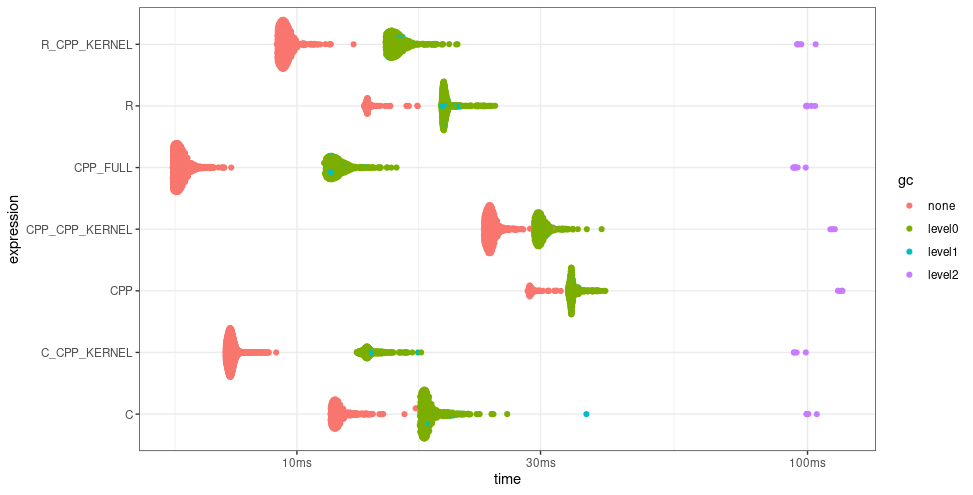
\includegraphics[scale = 0.5]{figure/CVsRcppDensity.png}
  \end{figure}
\end{frame}
\begin{frame}
  \frametitle{Benchmarking All Density Calculation Implementations}
  \framesubtitle{Table}
  \begin{figure}
    \centering
    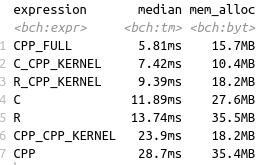
\includegraphics[scale = 0.7]{figure/CvsRCPPvsR_dens.png}
  \end{figure}
\end{frame}
\begin{frame}
  \frametitle{Benchmarking All LOOCV Implementations}
  \framesubtitle{Plot}
  \begin{figure}
    \centering
    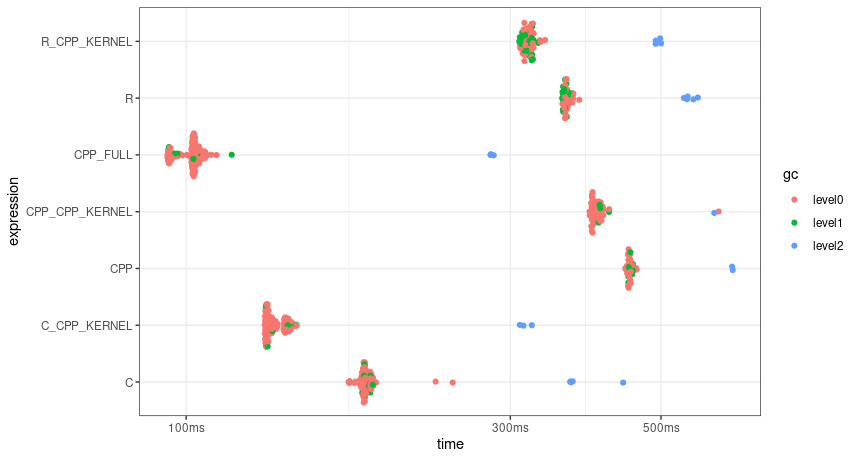
\includegraphics[scale = 0.5]{figure/CVsRcpBandwidth.png}
  \end{figure}
\end{frame}
\begin{frame}
  \frametitle{Benchmarking All LOOCV Implementations}
  \framesubtitle{Table}
  \begin{figure}
    \centering
    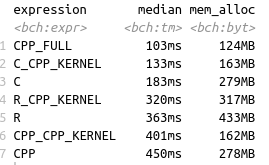
\includegraphics[scale = 0.7]{figure/CvsRCPPvsR_cv.png}
  \end{figure}
\end{frame}
\begin{frame}[fragile]
  \frametitle{Final implementation}
\begin{minted}{r}
dens <- function(x,
                 kernel,
                 bandwidth = bw_cv,
                 ...,
                 points = 512L) {
  if(is.function(bandwidth)) {
    bw <- bandwidth(x, kernel, ...)
  } else {
    bw <- bandwidth
  }
  p <- seq(min(x) - bw, max(x) + bw, length.out = points)
  y <- .Call("C_dens", x, p, kernel, bw, environment())
  structure(
    list(
      x = p,
      y = y,
      bw = bw
    ),
    class = "dens"
  )
}
\end{minted}
\end{frame}
\end{document}
